\documentclass[tikz,border=10pt]{standalone}
\usepackage{tikz}
\usetikzlibrary{shapes,arrows,positioning,fit,backgrounds}

\begin{document}
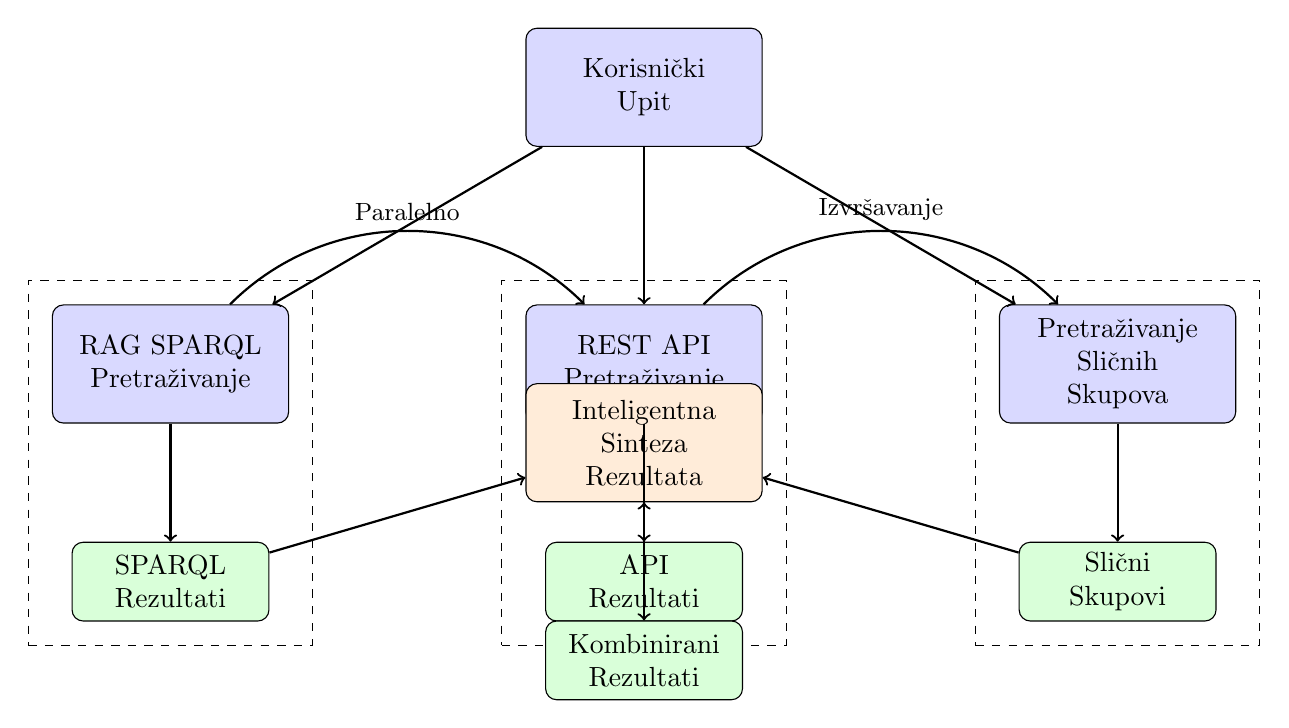
\begin{tikzpicture}[
    node distance=2cm,
    strategy/.style={rectangle, draw, rounded corners, minimum width=3cm, minimum height=1.5cm, align=center, fill=blue!15},
    result/.style={rectangle, draw, rounded corners, minimum width=2.5cm, minimum height=1cm, align=center, fill=green!15},
    synthesis/.style={rectangle, draw, rounded corners, minimum width=3cm, minimum height=1.5cm, align=center, fill=orange!15},
    arrow/.style={->, thick},
    label/.style={font=\small}
]

% User query
\node[strategy] (query) {Korisnički\\Upit};

% Search strategies
\node[strategy, below left=2cm and 3cm of query] (sparql) {RAG SPARQL\\Pretraživanje};
\node[strategy, below=2cm of query] (api) {REST API\\Pretraživanje};
\node[strategy, below right=2cm and 3cm of query] (similar) {Pretraživanje\\Sličnih\\Skupova};

% Results
\node[result, below=1.5cm of sparql] (sparql_results) {SPARQL\\Rezultati};
\node[result, below=1.5cm of api] (api_results) {API\\Rezultati};
\node[result, below=1.5cm of similar] (similar_results) {Slični\\Skupovi};

% Synthesis
\node[synthesis, below=3cm of query] (synthesis) {Inteligentna\\Sinteza\\Rezultata};

% Final output
\node[result, below=1.5cm of synthesis] (final) {Kombinirani\\Rezultati};

% Background grouping
\begin{scope}[on background layer]
    \node[fit=(sparql)(sparql_results), draw, dashed, inner sep=0.3cm, label=above:Strategija 1] {};
    \node[fit=(api)(api_results), draw, dashed, inner sep=0.3cm, label=above:Strategija 2] {};
    \node[fit=(similar)(similar_results), draw, dashed, inner sep=0.3cm, label=above:Strategija 3] {};
\end{scope}

% Main flow arrows
\draw[arrow] (query) -- (sparql);
\draw[arrow] (query) -- (api);
\draw[arrow] (query) -- (similar);

% Strategy to results
\draw[arrow] (sparql) -- (sparql_results);
\draw[arrow] (api) -- (api_results);
\draw[arrow] (similar) -- (similar_results);

% Results to synthesis
\draw[arrow] (sparql_results) -- (synthesis);
\draw[arrow] (api_results) -- (synthesis);
\draw[arrow] (similar_results) -- (synthesis);

% Final output
\draw[arrow] (synthesis) -- (final);

% Parallel execution indicator
\draw[arrow, bend left=45] (sparql) to node[label, above] {Paralelno} (api);
\draw[arrow, bend left=45] (api) to node[label, above] {Izvršavanje} (similar);

\end{tikzpicture}
\end{document} 